\documentclass[12pt,oneside]{book}

\usepackage[foundations, settheory]{../../lib/tex/naproche}
\usepackage{../../lib/tex/libraries}
\usepackage{graphicx}
\usepackage{float}
\usepackage{caption}


\title{Set theory}
\author{Marcel Schütz}
\date{2022}

\begin{document}
  \maketitle

  \tableofcontents

  \paragraph*{}
  \begin{figure}[H]
    \centering
    \fbox{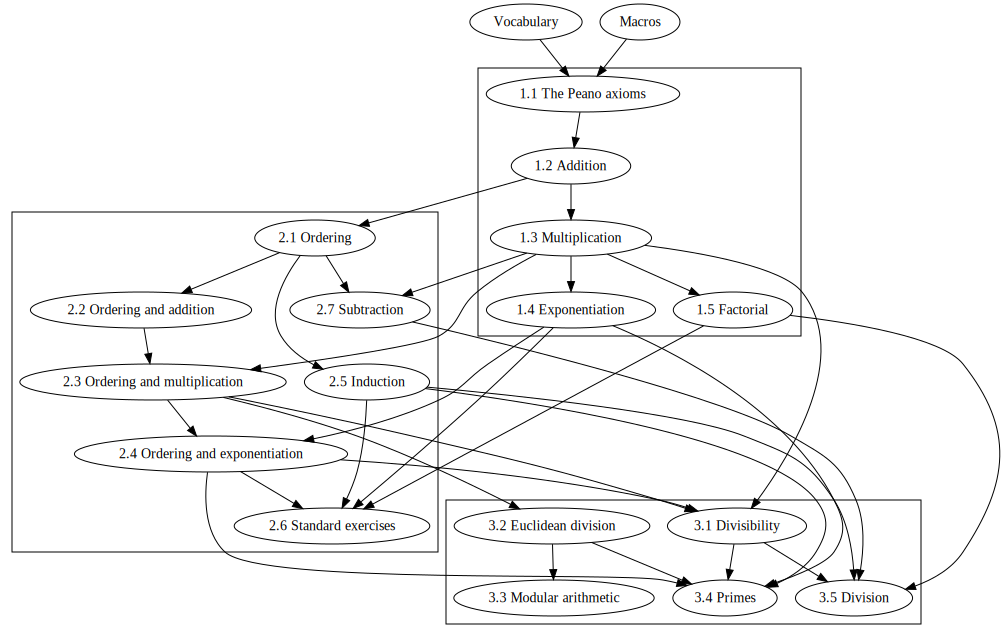
\includegraphics[width=0.9\textwidth]{./dependency-graph/graph.png}}
    \caption*{Interdependencies of the chapters}
  \end{figure}

  \section*{Introduction}

  This is a library providing basic results from undergraduate-level set theory.
  It introduces the notion of transitive classes
  (\cref{chapter:transitive-classes}), defines the notion of ordinal numbers
  (\cref{chapter:ordinals}) and as a special case of the latter introduces the
  set $\omega$ of finite ordinals (\cref{chapter:finite-ordinals}).
  Moreover, this library provides a formalization of the ordinal recursion
  theorem (\cref{chapter:recursion}) which is used to prove Zermelo's
  well-ordering theorem (\cref{chapter:zermelo}), on the basis of which the
  notion of cardinal numbers is introduced (\cref{chapter:cardinals}).

  \paragraph*{Usage.}
  At the very beginning of each chapter you can find the name of its source
  file, e.g. \path{set-theory/sections/01_transitive-classes.ftl.tex} for
  \cref{chapter:transitive-classes}.
  This filename can be used to import the chapter via \Naproche's
  \texttt{readtex} instruction to another ForTheL text, e.g.:
  \begin{center}
    \verb`[readtex \path{set-theory/sections/01_transitive-classes.ftl.tex}]`
  \end{center}

  \paragraph*{Checking times.}
  The checking times for each of the chapters may vary from computer to
  computer, but on mid-range hardware they are likely to be similar to those
  given in table below:

  \begin{center}
    \begin{tabular}{c|c|c}

      & \multicolumn{2}{c}{\textbf{Checking time}}
      \\
      \textbf{Chapter}
      & \textbf{without dependencies}     & \textbf{with dependencies}
      \\ \hline
      \ref{chapter:transitive-classes}
      & 00:20 min                         & 07:00 min
      \\
      \ref{chapter:ordinals}
      & 03:20 min                         & 10:30 min
      \\
      \ref{chapter:finite-ordinals}
      & 01:15 min                         & 11:45 min
      \\
      \ref{chapter:recursion}
      & 04:05 min                         & 14:35 min
      \\
      \ref{chapter:zermelo}
      & 04:45 min                         & 21:40 min
      \\
      \ref{chapter:cardinals}
      & 05:10 min                         & 26:50 min
    \end{tabular}
  \end{center}

  \subfile{sections/01_transitive-classes.ftl.tex}
  \subfile{sections/02_ordinals.ftl.tex}
  \subfile{sections/03_finite-ordinals.ftl.tex}
  \subfile{sections/04_recursion.ftl.tex}
  \subfile{sections/05_well-ordering-theorem.ftl.tex}
  \subfile{sections/06_cardinals.ftl.tex}
\end{document}
